
%======================ģ�ͽ���====================================
\section{Introduction}
A lot of numbers are usually used to describe the career of a coach in different sports: total years, matches, victories, winning percentage, champoinships, and so on. There also exist other factors that cannot be directedly obtained by these simple data, or even cannot be reflected by \textbf{any} data. These facts make it almost impossible to propose a perfect assessment method for college coaches.



Our goal is to build a mathematical model to find the best all time college coach or coaches in the previous century in certain sports. Here we mainly focus on NCAA Men's basketball, football,

In our metrics for assessment, we use 4 parameters

We develop 2 parameters that can reveal the ability of a coach. Promotion   Stability      Our metric attaches high importance to these aspects.   based on the performance of the team he is managing



 inside the conference it belongs to
%Assessing a college coach can be hard. Traditionally, the assessment of a coach is entirely decided by the  performance of his team. This method, however, is not convincing enough in that it neglects the promotion a coach has brought to his team.

We, on the other hand, develop a model trying to combine these two aspects together by taking both these two elements, performance of the team and promotion brought by the coach, into consideration. Furthermore, we develop a method to evaluating the performance of a team with limited information, which makes the evaluation for coaches of the whole past century possible since data in those early years may not be as comprehensive as it is now.


%Although a hitter might expect a model of the bat?Cbaseball collision to
%yield insight into how the bat breaks, how the bat imparts spin on the ball,
%how best to swing the bat, and so on, we model only the sweet spot.


%=============================����ģ��==========================================
\section{Framework of the Model}
Basically, our model assesses a coach based on the performance of teams.











In order to find the promotion and stability of a coach, a fundamental issue here is to properly evaluate the performance of a team in a season. This issue, however, is related to several aspects which are intricately connected with each other. Based on the competetion system of NCAA, our model develops a method to give an assessment of the performance for the team based on its Win-Loss percentage in the regular season inside the conference it belongs to     , its opponents' strength and the strength of conference it is in.






In the evaluation of the performance of a team in a single year, we consider its matching results in the regular season, and also estimate the overall strength of this conference and the intensi

Based on a comprehensive evaluation of performance for all teams, the model get some parameters which can depict different aspects of a coach. These parameters are carefully selected such that they are independent of each other and each parameter is well related to an aspect of the coach. Besides, these parameters will make full use of our data found, which suggests the comprehensiveness of our model.

A series of preliminaries are set to filter coaches ahead of the model in order to minimize our size of candidates. These preliminaries are selected such that real "legends" will not be overlooked and will sure to be selected. This procedure will greatly alleviate our calculation, thus making more comprehensive and complicate model possible.

The model can be explained by \textbf{Figure 1}:
\begin{figure}[!ht]
\centering
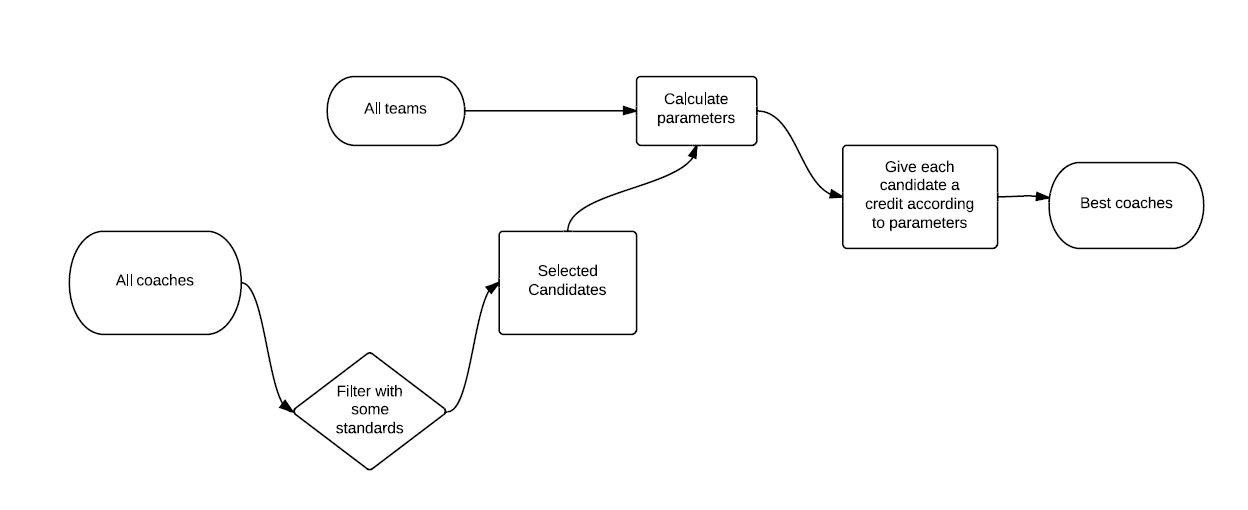
\includegraphics[width = 150mm]{picture/OverallFrame.png}
\caption{Overall framework}
\end{figure}

In the model, based primarily on records of NCAA teams for the last century, we synthesize the data into two parameters: performance and promotion.

Performance measures the team's performance during the time directed by the coach of interest. This parameter is similar to the traditional way of measurements. Promotion measures to what extent did the coach enhanced the performance of the team. As will showed later, these two parameter is based on data of different periods of a team, so they do depict different aspects of a coach.

\section{Basic definitions}

\subsection{Win-Loss percentage}
Since the model's purpose is to rank coaches in the past century, records must be carefully selected to enable the comparison between teams from different era. We select Win-Loss percentage(WLP) as one of its basic figures.
\newtheorem{definition}{Definition}
\begin{definition}
Given a season of interest, suppose the team under consideration has $w$ wins, $l$ losses. The Win-Loss percentage(WLP) is:
$$WLP \doteq \frac{w}{w + l}.$$
\end{definition}

The selection is based on the following considerations:

\begin{itemize}
\item Win-Loss percentage for the sports we select is recorded or can be easily calculated throughout the whole past century.
\item Win-Loss percentage can minimize the influence brought by different tournament system and different rules, which provides the model with more generality.
\item For all teams, the Win-Loss percentage is of the same scale, which means $WLP\in [0,1]$.
\item The expectation for Win-Loss percentage is the same for all teams, which is 0.5. So this is a fair index when comparing performances across teams, avoiding prejudices brought by the model.
\end{itemize}

\subsection{Conference Strength}
Besides records for a single team, the model also considers the strength of the conference the team is in. By this number we estimate the overall strength of teams in a conference and can be used to compare teams from different conferences.
\begin{definition}
In a season of interest, the teams in a conference have a total of $W$ wins, $L$ losses, $D$ ties against the teams from other conferences. Then its \textbf{Conference Strength} $p$ is
$$p = \frac{W}{W+L}.$$
\end{definition}

%Here overall wins(losses, ties) means all games, whether the opponents are from the same conference or not, is taken into consideration, and conference wins(losses, ties) only considers those games with opponents in the conference.

Note that it is similar to the definition of WLP, so this parameter has similar properties as WLP:
\begin{itemize}
\item Conference Strength for the sports we select can be calculated throughout the whole past century.
\item Conference Strength is related to the overall performance of teams in a conference, and does not necessarily related to tournament system and rules, which provides the model with more generality.
\item For all conferences, Conference Strength is of the same scale, which means $p\in [0,1]$.
\item The expectation for Conference Strength is the same for all conferences, which is 0.5. So this is a fair index when comparing performances across conferences, avoiding prejudices brought by the model.
\end{itemize}

%==================================��������==============================================

\subsection{Measurement for Performance}
In this part, we will explain the method to measure a team's performance. This number will serve as a basic part for evaluating promotion and stability. For the team, we're interested in its WLP of all conference games in the regular season.

\newcommand{\performance}{x_i\frac{1+b(p-0.5)}{1+a\sigma}}
\begin{definition}
In a season of interest, suppose there are N teams in a conference $t_1, t_2,\dots,t_N$. Team $t_i$ has a WLP $x_i$. The conference has a Conference Strength $p$. Then the performance for team $t_i$ is
$$y_i\doteq \performance.$$
\end{definition}

Here $\sigma$ is the standard deviation of $x_1, x_2, \cdots, x_N$, which is $\sigma = \sqrt{ \frac{\sum_{i=1}^{N}(x_i - \mu)^2}{N}}$ and $\mu = \frac{\sum_{i=1}^N{x_i}}{N}$. Thus $\sigma$ is used to estimate the intensity of competition inside this conference. The smaller $\sigma$ is, the more intense is the inner competition.

In the definition, $a$ and $b$ are both tunable positive parameters and both should be relatively small. %In fact, here $a$ depicts the influence of the team's opponents and $b$ depicts the influence of the conference.

The definition of $y_i$ has the following properties:

\newtheorem{property}{Property}

\begin{property}
$$\frac{\partial{y_i}}{\partial{x_i}} > 0$$
\end{property}
\begin{comment}
\begin{proof}
$$\frac{\partial{y_i}}{\partial{x_i}} = \frac{1+b(p-0.5)}{1+a\sigma}$$
Since both $a$ and $b$ are positive, we have $\frac{\partial{y_i}}{\partial{x_i}}>0$.
\end{proof}
\end{comment}

\begin{property}
$$\frac{\partial{y_i}}{\partial{\sigma}}<0$$
\end{property}
\begin{comment}
\begin{proof}
$$\frac{\partial{y_i}}{\partial{\sigma}} = -x_i\frac{1+b(p-0.5)}{1+a\sigma}\ln(1+a\sigma)$$
Similarly, we have both $a$ and $b$ are positive, so $\frac{\partial{y_i}}{\partial{\sigma}}<0$
\end{proof}
\end{comment}

\begin{property}
$$\frac{\partial{y_i}}{\partial{p}} > 0$$
\end{property}
\begin{comment}
\begin{proof}
$$\frac{\partial{y_i}}{\partial{\p}} = \frac{b}{1+a\sigma}x_i > 0$$
\end{proof}
\end{comment}

These three properties are easy to observe and they suggest how performance is related to three variables. Then the team's performance is based on its WLP, and should be scaled up with the increase of the conference strength and intensity. Specifically, since $p=0.5$ means the conference is of average level among all conferences, there is a $(p-0.5)$ inside the definition to be consistent with this property.


We choose appropriate values for $a$ and $b$ to make this measurement be consistent among all conferences and all eras. The expectation of $y_i$ is close to 0.5 given that $a$ and $b$ are both small. So $\sigma$ and $p$ will not bring into the model too much prejudices but only minor amendments.


%Next we have \textbf{Property 4}, which will guarantee the comparable between different teams from different conferences or/and different eras.
%\begin{property}
%$$\frac{\sum_{i=1}^N{y_i}}{N}<\frac{1-b}{2(1+a)}$$
%\end{property}

%To prove \textbf{Property 4}, first we prove the following claim:
%\newtheorem{claim}{Claim}

%\begin{claim}
%In a tournament with N teams $t_1,t_2,\dots,t_N$, team $t_i$ has a WLP $x_i$, then
%$$\sum_{i=1}^N{x_i} = \frac{N}{2}$$
%\end{claim}
%\begin{proof}
%Each team plays the same number of games, which is $2N\choose 2=N(N-1)$, suppose team $t_i$ has $w_i$ wins and $d_i$ ties. Then
%$$x_i=\frac{w_i + 0.5t_i}{N(N-1)}$$
%so
%$$\sum_{i=1}^N{x_i} = \frac{\sum_{i=1}^N(w_i + 0.5t_i)}{N(N-1)}$$
%Since each game is counted either as a win and a loss or as two ties, we have
%$$\sum_{i=1}^N(w_i+0.5t_i)=\frac{N(N-1)}{2}$$
%so we have
%$$\sum_{i=1}^N{x_i} = \frac{N}{2}$$
%\end{proof}

%Then we can prove \textbf{Property 4}
%\begin{proof}
%\begin{align}
%\sum_{i=1}^Ny_i &= \frac{1+b(p-0.5)}{1+a\sigma}\sum_{i=1}^Nx_i\\
%&=\frac{1+b(p-0.5)}{1+a\sigma}\frac{1}{2}\\
%&<\frac{1-b}{2(1+a)}
%\end{align}
%\end{proof}

\textbf{Comparison with SRS}

Here we compare our measurements with another system of performance measurement called simple ranking system(SRS), which is used for ranking college basketball teams recently in National Collegiate Athletic Association(NCAA).

SRS is aimed at involving opponent's performance into a single team's assessment and finally make reliable predictions about which team will get the most credits in the conference. Different from our model, SRS builds its evaluation on a set of equations
\begin{align}
\nonumber
&R_1 = x_1 - \mu + \frac{1}{N-1}\sum_{j\neq i} R_j\\\nonumber
&R_2 = x_2 - \mu + \frac{1}{N-1}\sum_{j\neq i} R_j\\\nonumber
&...\\\nonumber
&R_N = x_N - \mu + \frac{1}{N-1}\sum_{j\neq i} R_N \\\nonumber
\end{align}
where $\mu = \frac{\sum_{i=1}^Nx_i}{N}$

This set of equations can be solved with Gauss-Seidel algorithm. Obviously, there are two parts in each equation. The first one is $x_i - \mu$, which stands for credits got by the team. Another part is  $\frac{1}{N-1}\sum_{j\neq i} R_j$, which can be seen as an amendment brought by its opponents.

This method, however, cannot achieve its initial purpose. Further study shows that this set of equations has a solution set like
$$R_i = \frac{N-1}{N}x_i + c$$
where $c$ is an arbitrary constant.

So what we got from this method only relies on N and $x_i$, instead of $x_1, x_2,\dots,x_N$ as we wished. In contrast, our model do take every team's WLP into consideration, which suggests this method can partly shows the relationships among different teams inside the conference.

Also, our measurement takes into account the overall performance of the conference while SRS does not. So SRS cannot be applied to compare teams from different conferences.

\subsection{$PRM(c)$}
The calculations of $PRM(c)$ and $STB(c)$ are based the above definition of performance of a team in a specific season. To make it clear, we denote it by $PERF(t, s)$, where $t$ is the team, and $s$ is the season.

%The promotion is determined by two parts of data. One is the team's \emph{historical performance}, which means how this team works before the coach came to the team and another is the team's \emph{temporary performance}, which shows how the team works during the period directed by the coach. The model makes a prediction based on the historical performance and compares the prediction with its real performance. The result of the comparison will be used as promotion.
For a coach $c$, we first choose a team $t$ that he has coached. If he has only coached one team in his career, then $t$ is this team. If he has coached more than one team, we choose the one that he has coached for the longest time.

Suppose $C$ coached $t$ in seasons $s_1, s_1+1, \cdots, s_2$.

Let the average performance of $t$ in the first $r$ seasons coached by $c$ $s_1, s_1+1, \cdots, s_1+r-1$ be $P_{after}$, and the average performance of $t$ in the last $r$ seasons before $C$'s coaching be $P_{before}$. Here $r$ is a constant to be chosen. Let $PRM(c)=P_{after}-P_{before}$. To make it clear:
\begin{definition}
$$PRM(c)= \frac{\sum_{i = 1}^{r}PERF(t, s_1+i-1)}{r}-\frac{\sum_{i = 1}^{r}PERF(t, s_1-r)}{r}.$$
\end{definition}

%\begin{definition}
%Suppose we have a team's historical performance $y_1, y_2,\dots, y_s$ and its temporary performance $y_{s+1}, y_{s+2},\dots, y_r$. Then the promotion is
%$$p\doteq \frac{\sum_{i = s+1}^ry_i}{r-s} - \frac{\sum_{i=1}^sy_i}{s}$$
%\end{definition}

This definition of promotion is straightforward. This difference descibes the promotion that the coach brought to this team.

Note that when calculating $PRM(c)$, a lot of information is used other than those are obviously related to $c$, which suggests the model is more comprehensive. Since the data we can use are limited because of the long time interval, taking full use of data is an advantage of our model.

\subsection{$STB(c)$}
\begin{definition}
Let $STB(C)$ be the standard deviation of $PERF(t, s_1), PERF(t, s_1+1), \cdots, PERF(t, s_2)$.
\end{definition}

This is also easy to understand. We use the standard deviation of the team's performances to estimate $STB(c)$.
%===============================�ۺϷ���============================================
\section{Synthesized Evaluation Based on Four Aspects}
In this section, we will give an overall credit for a coach based on his performance in four aspects discussed in previous section. For a coach c, $PRM(c)$, $STB(c)$, $ACH(c)$ and $WLP(c)$ will be summed up with weights decided by analytic hierarchy approach.

The hierarchy for this problem is shown in \textbf{Figure 2}
\begin{figure}[!hf]
\centering
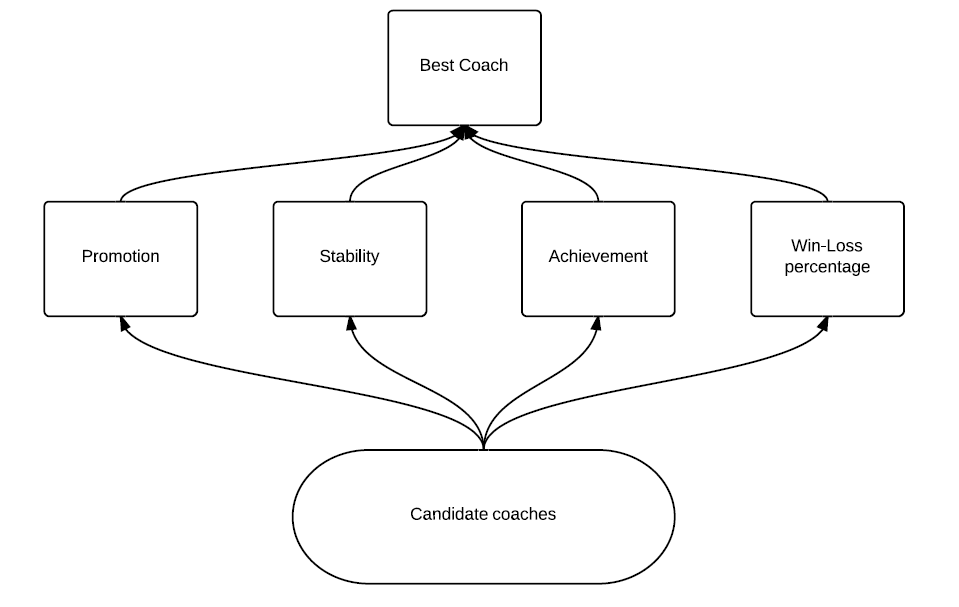
\includegraphics[width = 150mm]{Hierarchy.png}
\caption{Hierarchy}
\end{figure}

Based on this hierarchy, we have the following comparison matrix
$$
\left(
  \begin{array}{cccc}
    1 & \frac{1}{3} & \frac{1}{7} & \frac{1}{5} \\
    3 & 1           & \frac{1}{3} & \frac{1}{3} \\
    7 & 3           & 1           & 3           \\
    5 & 3           & \frac{1}{3} & 1           \\
  \end{array}
\right)
$$

Now we verify the matrix
\begin{align}
CI &= \frac{\lambda_{MAX}(A) - 4}{3}\nonumber\\
\lambda_{MAX} &= 4.13973 \nonumber\\
RI &= 0.90\nonumber
\end{align}

So $CR = \frac{CI}{RI}=0.052 < 0.1$, the matrix can be used as comparison matrix.

Then we have its eigenvectors is $(0.056, 0.139, 0.525, 0.280)^T$.

Now we have the synthesized credit defined as following

\begin{definition}
For a coach $c$, the synthesized credit is
$$EVA(c) = 0.056PRO(c) + 0.139STA(c) + 0.525ACH(c) + 0.280WLP(c)$$ 
\end{definition}

%========================ģ�ͽ��============================

\section{Validating the Model}
Although Mr. Gore has expressed concerns to some associates about
the damage a brokered convention could cause, several associates
said he was hopeful that one candidate would soon break through,
sparing the party such an outcome. He told a close friend recently
that his decision not to endorse ??feels like the right thing??
and that he remained optimistic the race ??is going to tip at some
point,?? the friend said. Although Mr. Gore has expressed concerns
to some associates about the damage a brokered convention could
cause, several associates said he was hopeful that one candidate
would soon break through, sparing the party such an outcome. He
told a close friend recently that his decision not to endorse
??feels like the right thing?? and that he remained optimistic the
race ??is going to tip at some point,?? the friend said.


Although Mr. Gore has expressed concerns to some associates about
the damage a brokered convention could cause, several associates
said he was hopeful that one candidate would soon break through,
sparing the party such an outcome. He told a close friend recently
that his decision not to endorse ??feels like the right thing??
and that he remained optimistic the race ??is going to tip at some
point,?? the friend said.

\section{Conclusions}
Although Mr. Gore has expressed concerns to some associates about
the damage a brokered convention could cause, several associates
said he was hopeful that one candidate would soon break through,
sparing the party such an outcome. He told a close friend recently
that his decision not to endorse ??feels like the right thing??
and that he remained optimistic the race ??is going to tip at some
point,?? the friend said.
\section{A Summary    }
Although Mr. Gore has expressed concerns to some associates about
the damage a brokered convention could cause, several associates
said he was hopeful that one candidate would soon break through,
sparing the party such an outcome. He told a close friend recently
that his decision not to endorse ??feels like the right thing??
and that he remained optimistic the race ??is going to tip at some
point,?? the friend said.
%================================ģ������==============================
\section{Evaluate of the Mode}

%======================================================================
\section{Strengths and weaknesses}
Like any model,the one present above has its strengths and
weaknesses. Some of the major points are presented below.

%============================ģ����ȱ��====================================
\subsection{Strengths}
\begin{itemize}
\item \textbf{Applies widely}\\
This  system can be used for many types of airplanes, and it also
solves the interference during  the procedure of the boarding
airplane,as described above we can get to the  optimization
boarding time.We also know that all the service is automate.
\item \textbf{Improve the quality of the airport service}\\
Balancing the cost of the cost and the benefit, it will bring in
more convenient  for airport and passengers.It also saves many
human resources for the airline. \item \textbf{}
\end{itemize}




\begin{thebibliography}{99}
\addcontentsline{toc}{section}{References}
\bibitem[D. E. KNUTH]{1} D. E. KNUTH   The \TeX{}book  the American
Mathematical Society and Addison?CWesley
Publishing Company , 1984-1986.
\bibitem{2}Lamport, Leslie,  \LaTeX{}: `` A Document Preparation System '',
Addison-Wesley Publishing Company, 1986.
\end{thebibliography}

%====================???????????????==========================================
    \begin{appendices}
    %\renewcommand{\thesection}{\Alph{chapter}.}

      \section{First appendix}

    some text...


Here are simulation programmes we used in our model as follow.\\


\textbf{\textcolor[rgb]{0.98,0.00,0.00}{Input matlab source:}}
\lstinputlisting[language=Matlab]{./code/matlab1.m}


      \section{Second appendix}

    some more text\textcolor[rgb]{0.98,0.00,0.00}{\textbf{Input C++ source:}}
\lstinputlisting[language=C++]{./code/sudoku.cpp}

    \end{appendices}
